\section{nRF24L01}
The following section contains the tests performed on the nRF24L01 radio module. These tests were performed to determine different properties of the radio module, such as range and reliability.

\subsection{Range}
A basic test was performed to assess the range of the radio module, to ensure they are usable in a practical application. 

The testing was done by having two units set as transmitter and receiver units respectively, having the transmitter repeatedly sending a single signal while increasing the distance between the units. When the receiver no longer received the signal, the distance was measured.

This test showed a range of about 160 meters without obstacles, although the number of successfully transmitted packets declined the longer the distance.

\subsection{Bit Error Rate Test}
When transmitting data from one unit to another, it is important that the data is correct. To get an idea of how much error is introduced during the communication, a bit error test was performed, hereby referenced to as BERT.

\subsubsection*{About BERT}
The basic concept of BERT is to send a known data stream from one unit to another, and check how much it differs from the expected data stream.

The duration of a BERT should vary depending on the results. To get an exact result it would take an infinite amount of time, which is not feasible. But due to the nature of randomness, if only a small amount of errors are met, then it could just be a lucky test, so the testing length would have to be sufficiently long for getting a general idea of the average error rate. Because of this, multiple BERT runs were executed.

\subsubsection*{Executing BERT} 
The test was executed by sending packets from an Arduino to a Raspberry Pi, using the nRF24L01 modules.

The code ran on the devices for the test can be found in Appendix \ref{cha:bertcode}. The sender code transmits some deterministic value, and the receiver checks whether the received packet is the same as the one expected. If the two packets match, the 'successes' value is incremented, if not, the 'errors' value is incremented.

The BERT was executed four times. The first three times with 1.000.000 packets transmitted, and the fourth time with 10.000.000 packets. For every 1.000 packet received, the number of errors and successes were printed for those 1.000 packets. 
The values were then imported into a spreadsheet for statistics.
The complete spreadsheet with results and graphs can be found on the attached DVD. 

\subsubsection*{Result of BERT}
The results of the BERT showed a packet failure of under one percent. Some spikes were present in the test results, with the highest being at 797 missed packets, which occured in the first test, as seen in figure \ref{fig:bert1}.

\begin{figure}[h!]
\hspace*{-2cm}
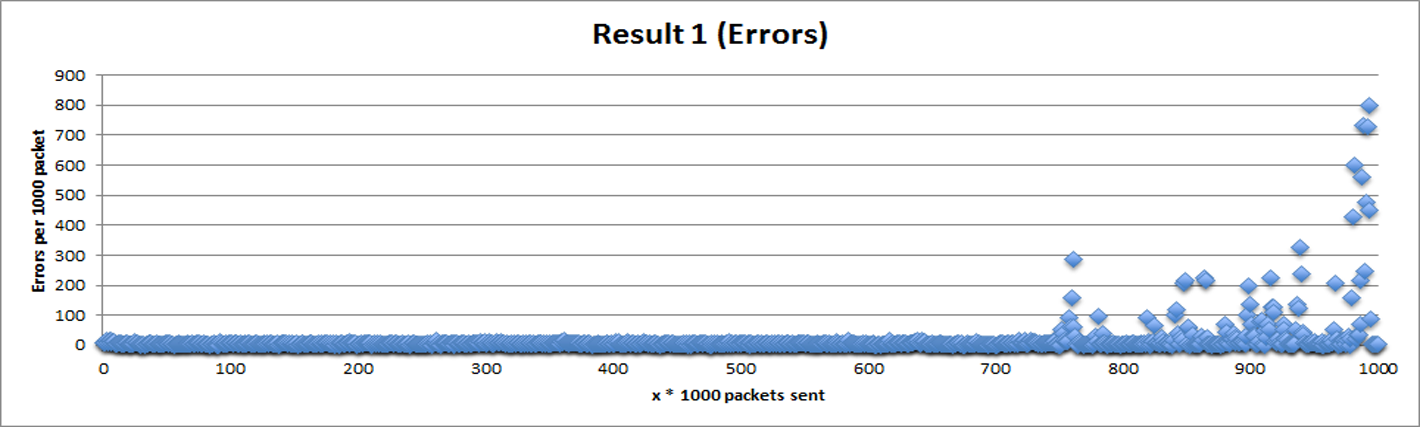
\includegraphics[width=1.3\textwidth]{chapters/test/figures/res1.png}
\caption{Graph representing the first BERT run.}
\label{fig:bert1}
\end{figure}

The three last tests generally had a lower number of missed packets. Test number two had a peak of 304 lost packets, as seen in figure \ref{fig:bert2}, and test three had a peak of 340 lost packets, figure \ref{fig:bert2}. Test four had a peak of 163 lost packets, seen in figure \ref{fig:bert3}.

\begin{figure}[h!]
\hspace*{-2cm}
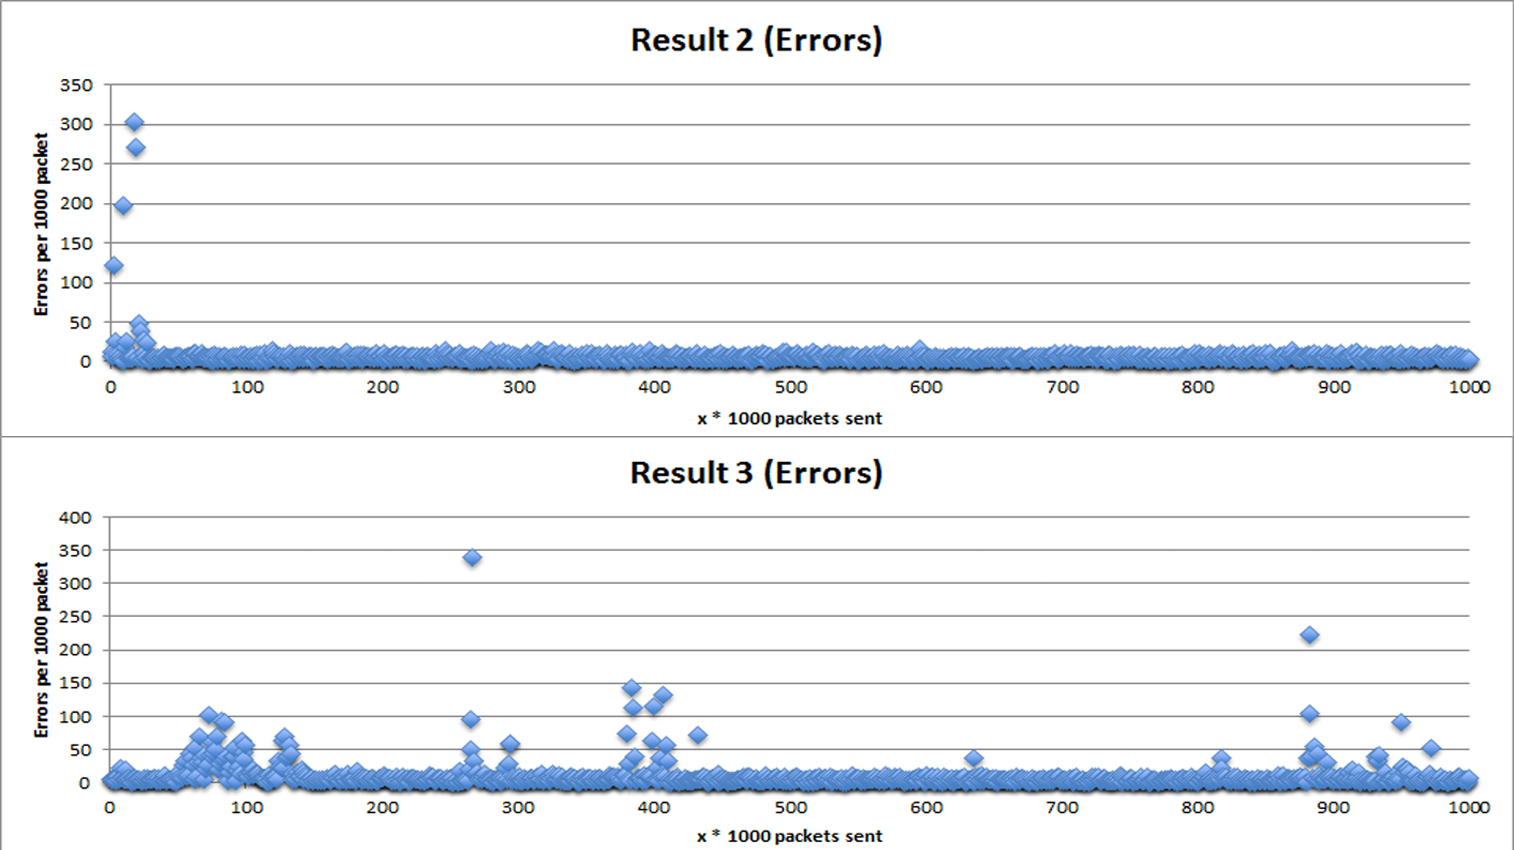
\includegraphics[width=1.3\textwidth]{chapters/test/figures/res5.png}
\caption{Graph representing the second and third BERT run.}
\label{fig:bert2}
\end{figure}

As seen in the first and second test in figure \ref{fig:bert2}, the high number of errors occurred in clusters. This could be attributed to the time of the testing, where other groups might have been testing wireless modules, or some other source of interference occurred.

Most of the tests were high in success, and low on failures. In the first run, the average failed packets per 1.000 was at 16.5. The second run had an average of 6.4 failed per 1.000. Third run had 9.3 failed per 1.000 and the fourth run had 7.2 failed per 1.000.\todo{tablify!}


\begin{figure}[h!]
\hspace*{-2cm}
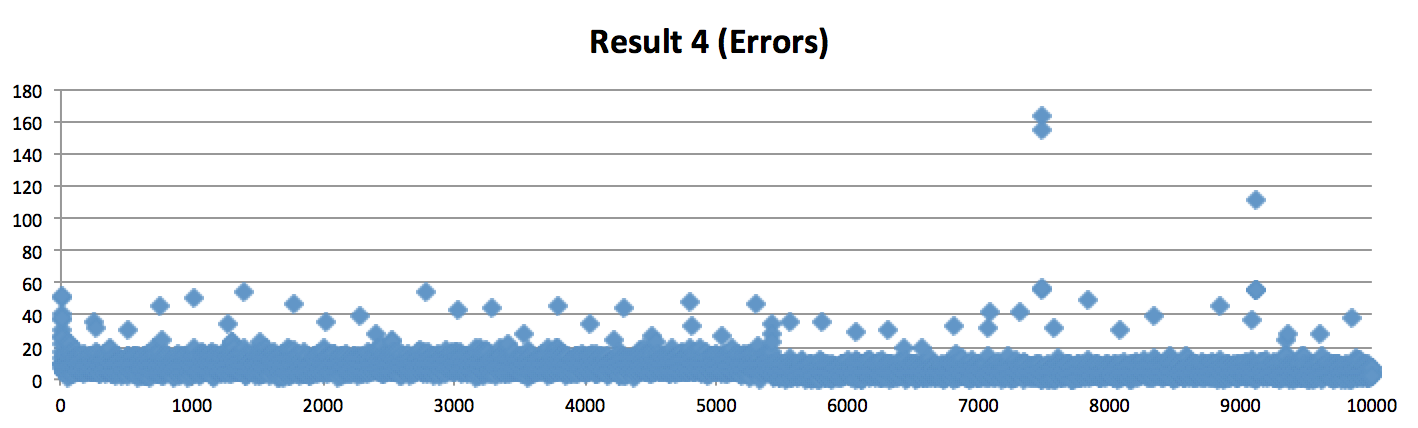
\includegraphics[width=1.3\textwidth]{chapters/test/figures/res4.png}
\caption{Graph representing the fourth BERT run.}
\label{fig:bert3}
\end{figure}

The fourth run was performed using ten million packets, and the graph provides better insight on the randomness of errors. A few peaks appeared, but usually smaller peaks between 40 and 60 packets lost per 1.000.

Generally, the error count is low and even regarding the pikes, and the module seems stable. On a golf course, there will not be the same level of interference as in the group room, surrounded by wireless networks, phones, bluetooth devices and other sources of interference.

%primarysource http://www.radio-electronics.com/info/rf-technology-design/ber/bit-error-rate-testing-bert.php
